% Template for CAD in medical imaging - Project Report
%          spconf.sty  - ICASSP/ICIP LaTeX style file, and
%          IEEEbib.bst - IEEE bibliography style file.
% --------------------------------------------------------------------------
\documentclass{article}
\usepackage{spconf,amsmath,graphicx}
\usepackage{subfigure}

% Title
\title{Computer Aided Diagnosis\\LUNA16: False Positive Reduction}
%
\makeatletter
\def\@name{ \emph{Luc Nies (s4136748)}, \emph{Tom van de Poll (s4106512)}, \emph{Harmen Prins (s4132297)}, \\ \emph{Steven Reitsma (s4132343)} \& \emph{Inez Wijnands (s4149696)}}
\makeatother

\address{Radboud University Nijmegen}
%
% For example:
% ------------
%\address{School\\
%	Department\\
%	Address}
%
% Two addresses (uncomment and modify for two-address case).
% ----------------------------------------------------------
%\twoauthors
%  {A. Author-one, B. Author-two\sthanks{Thanks to XYZ agency for funding.}}
%	{School A-B\\
%	Department A-B\\
%	Address A-B}
%  {C. Author-three, D. Author-four\sthanks{The fourth author performed the work
%	while at ...}}
%	{School C-D\\
%	Department C-D\\
%	Address C-D}
%
% More than two addresses
% -----------------------
% \name{Author Name$^{\star \dagger}$ \qquad Author Name$^{\star}$ \qquad Author Name$^{\dagger}$}
%
% \address{$^{\star}$ Affiliation Number One \\
%     $^{\dagger}$}Affiliation Number Two
%
\begin{document}
%\ninept
%
\maketitle
%


% Introduction
\section{Introduction}
\label{sec:intro}
For the \emph{LUng Nodule Analysis 2016 (LUNA16)} challenge, we want to detect pulmonary nodules in low-dose thoracic CT images as accurately as possible. Initially the challenge is separated into three different phases; lung segmentation, candidate detection and false positive reduction. For the first two phases, we tried two different approaches. Firstly, we used deep learning to create a network that could train on the images and could recognize areas of interest. For the first phase these areas were the lung regions, for the second these areas were possible nodules in the lung regions. This way, we could treat both phases as a segmentation problem and could use the same network. Secondly, we used a more traditional approach using image processing techniques like region growing and blob detection in the images to complete these phases.\\
\indent After the second phase, we had so far obtained marginally better results for the deep learning approach than the traditional approach. Therefore, we focus solely on our deep learning approach for the third phase.\\
\\
\indent As mentioned, the third phase of our lung nodule detection challenge is false positive reduction. Heretofore, we have focused on identifying as many possible candidates as possible to include all annotated nodules in our selection. Thus, we only aimed at a high recall, but did not care much for precision. In this phase, we aim to obtain both high recall and high precision. We approached this problem by going back to the initial candidate selection, instead of taking our candidates and making a subselection to reduce the false positives. By tuning our network parameters and trying different settings overall, we tried to achieve better initial candidate selection and thus not needing false positive reduction, merging the second and third phase of the challenge. \\
\indent Our approach and its results are explained in further detail in the following sections.
\vfill

% Method
\section{Method}\label{sec:method} 
We implemented two different types of networks; a 2D fully connected network and a 3D convolutional network. We describe these in the following.

\subsection{Fully convolutional networks}
\subsubsection{Lung segmentation post-processing}
We have made use of the segmentations created by the network in earlier phases of the project, in order to more carefully select training patches from the images for training. A small issue with the segmentations created by the network is that there is some noise surrounding the actual lung segmentation. In order to use these segmentations for patch selection, the noise has to be removed from the images. In order to remove the noise, we perform an connected component analysis with a very small 3d-6 neighborhood. This divides the noise next to the segmentations into a large number of small connected components, but still sees the lungs and one large connected component. After this step, only the largest component in the image is selected and used as the real segmentation. This method works for every image in the dataset.
\cite{long}

\subsubsection{Nodule detection}
\label{sec:fcn}


\subsubsection{False positive reduction}
The FCN produces many false-positive pixels, thus producing a low precision. However, those pixels are almost never clustered together. Consequently, it is possible to do a connected components analysis on the output of the network and remove all components with a volume below a threshold. This threshold can be set manually or optimized using a small part of the data set. The second option is a good idea for future work.

\subsubsection{Analysing results with FROC}
To transform raw pixel data to coordinates as required by the FROC analysis, the same connected components analysis as for the false positive reduction is applied, and the centre of every component is located. Then, the FROC analysis is performed with the nodule diameter as the distance threshold. This means that every prediction that falls within a nodule is counted as a true positive and otherwise as a false positive.

\subsection{3D convolutional networks}
Next to the fully convolutional network approach, we also tested a three-dimensional convolutional network approach.
This method is simpler than the fully convolutional network, but needs to have nodule candidates as its input.
As such, it is not able to propose candidates itself, but needs some other system to do that.
The idea of the network is simple: its input consists of a 40x40x26 voxel neighborhood where the center is the nodule candidate coordinate.
The output of the network is a softmax distribution over the labels: in this case 0 for no nodule or 1 for a true nodule.
The network uses three-dimensional convolution and pooling layers to accommodate for the three dimensions in the data.
Alternatively, one could use multiple slices of the 3D cube in different angles and combine them.
However, we found that a three-dimensional approach performed better.
An input size of 40x40x26 was chosen by looking at the nodule sizes.
Prior work has already analyzed this \cite{qidou}, and in Figure \ref{fig:nodulesizes} you can see the result.

\begin{figure}[tb]
	\centering
	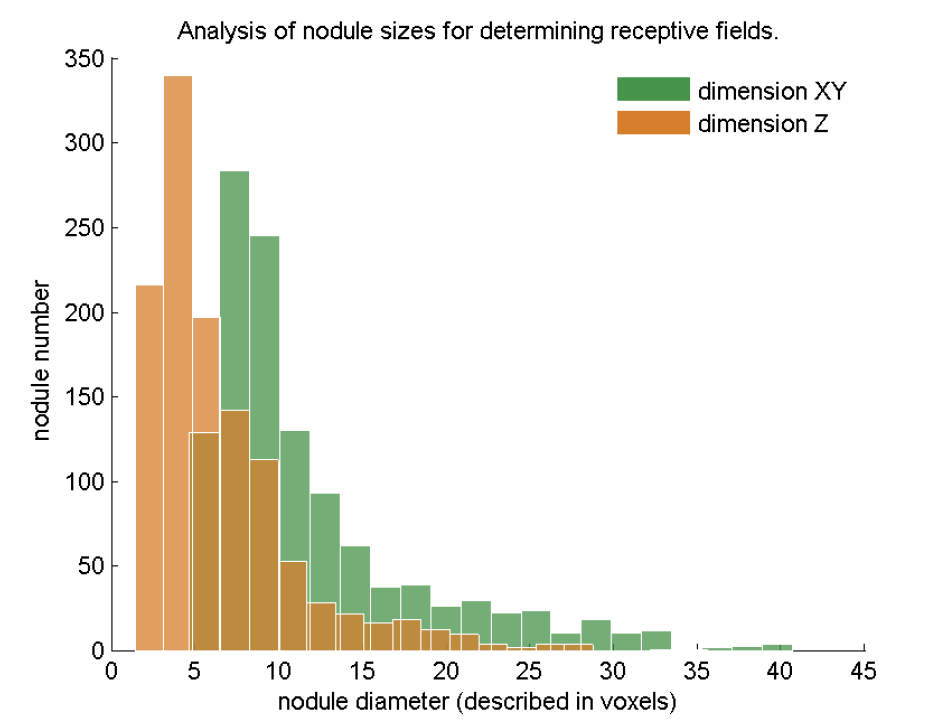
\includegraphics[width=0.45\textwidth]{nodulesizes.png}
	\caption{Analysis of the nodule sizes. Taken from \cite{qidou}.}
	\label{fig:nodulesizes}
\end{figure}

Just like in \cite{qidou}, we choose a smaller neighborhood in the Z dimension since its scaling is different from the other dimensions.
The network structure consists of four three-dimensional convolutional layers with a kernel size of 5x5x3.
After each convolutional layer, pooling is performed with a size and stride of 2x2x2.
Finally, two dense layers are added with 512 and 2 units respectively.
A softmax layer is applied to normalize the results and to obtain a probability distribution.
All layers have batch normalization and dropout is used in the first dense layer ($p=0.25$).
The network is trained using backpropagation with stochastic gradient descent and Nesterov momentum (0.9).
The learning rate is set to 0.001 and decays with 0.0001 per gradient step.
Binary cross-entropy loss was used and leaky ReLUs were used for every non-linearity in the network.
During training, each batch was balanced to contain approximately 50\% negative and 50\% positive classes.
Since there are a lot more negative examples, each epoch different negative examples are chosen and negative samples are never shown twice.
The network was implemented using Keras and Theano.
Proposed candidates are all taken from the extended false positive reduction csv file (candidates\_V2.csv) and evaluation was done using precision and recall metrics.
The network's results are shown in the results section.

% Experiments
%\section{Experiments}\label{sec:experiments}

% Results
\section{Results}\label{sec:results}
\subsection{3D convolutional network}
The results for the 3D convolutional network are shown in Table \ref{tbl:results_3d}.
\begin{table}[h!]
	\centering

	\begin{tabular}{l|cc}
	\hline

	\hline
	\textbf{Precision} & \textbf{Recall} & \textbf{$F_1$}\\
	\hline
		 0.87 & 0.92 & 0.89\\
	\hline

	\hline
	\end{tabular}
	\caption{Results for the 3D convolutional network.}
	\label{tbl:results_3d}
\end{table}

These results were computed on a separate validation set (15\% of data) without balancing.
While the scores look good, with more time we would have liked to perform 10-fold cross-validation and a FROC analysis to enable comparison to other LUNA2016 participants.
We also would have liked to add more data augmentation and to optimize the network structure.

\appendix
\section{Contributions}
\textbf{Luc Nies:} \\
\\
\textbf{Tom van de Poll:} Contributed to segmentation post-processing and wrote the report section on this topic\\
\\
\textbf{Harmen Prins:} Built connected components filter and FROC analysis. Wrote the corresponding sections.\\
\\
\textbf{Steven Reitsma:} Built the 3D convolutional network and wrote the report sections on this topic.\\
\\
\textbf{Inez Wijnands:} Access cluster. Wrote introduction section.

% References should be produced using the bibtex program from suitable
% BiBTeX files (here: strings, refs, manuals). The IEEEbib.bst bibliography
% style file from IEEE produces unsorted bibliography list.
% -------------------------------------------------------------------------
\bibliographystyle{IEEEbib}

\begin{thebibliography}{}
\bibitem{long}
J. Long, E. Shelhamer \& T. Darrell (2015). Fully convolutional networks for semantic segmentation. \emph{Proceedings of the IEEE Conference on Computer Vision and Pattern Recognition}: 3431--3440.

\bibitem{simonyan}
K. Simonyan \& A. Zisserman (2014). Very deep convolutional networks for large-scale image recognition. \emph{arXiv:1409.1556}

\bibitem{qidou}
Q. Dou, H. Chen \& P.A. Heng. Lung Nodule Classiffcation with Multi-level Contextual 3D Convolutional Neural Networks. \emph{Method description for LUNA2016}

%\bibitem{leemput}
%S. van de Leemput, F. Dorssers \& B.E. Bejnordi (2015). A novel spherical shell filter for reducing false positives in automatic detection of pulmonary nodules in thoracic CT scans. \emph{Proceedings SPIE Medical Imaging, 9414}:94142P.

\end{thebibliography}



\end{document}
